\section{Introduction}
Variational autoencoders (VAE), first introduced in the works of \cite{kingma2013autoencoding}, sparked a trend in designing generative models in order to approximate the intractable posterior distribution. Many recent papers have provided ingenious schemes for improving upon VAE, among some (\cite{iwae, rezende2015variational, ladder, kingma2018glow}), by achieving tighter log-likelihood bounds on the marginal likelihood (explained in greater detail below). The original bottom-up and top-down architecture has been experimented with (\cite{ladder}), as well as employing chains of transformations on an, in VAE, assumed simplistic prior distribution (\cite{rezende2015variational, kingma2018glow}). The importance weighted variational autoencoder (IWAE; \cite{iwae}) utilized averaging over multiple samples, as opposed to VAE's single-sample objective, to tighten the mentioned bound while being able to model a richer latent space – in effect, this multi-sample scheme allows for a more complex approximate posterior. In light of IWAE, tensor Monte-Carlo (\cite{tmc}; TMC) was recently proposed as an attempt to improve upon IWAE by sampling exponentially many importance samples. For each of the $n$ latent variables in the TMC, $K$ samples are drawn yielding $K^n$ marginal log-likelihood evaluations. Averaging over this large number of samples might appear computationally impossible, but via clever tensor products computed in parallel, the TMC is approximately as fast as the less importance sample exhausting IWAE. 

In this work, we reproduce what we believe are the most important results presented in the Tensor Monte Carlo paper (\cite{tmc}), where we also provide our reimplementation code. The original results in the TMC paper were attained via a PyTorch (\cite{pytorch}) implementation.\footnote{Code is available at:   \url{https://github.com/anonymous-78913/tmc-anon}.} In an attempt to ease understanding for those unfamiliar with PyTorch, we contribute with a TensorFlow\footnote{Code is available at:
\url{https://github.com/LinuNils/TMC_reproduced}.} (\cite{tensorflow}) implementation. Early on in our work, a connection was established with the author in order to bring our reproducibility work to their attention, as well as ensuring that we progress by clearing potential ambiguities. Due to resource and time constraints, we chose to reproduce those results that, in our meaning, appeared most informative and fundamental in the TMC paper. Additionally, as we found the TMC architecture non-trivial to understand, we aim to ease understanding for future users by complementing the textual description of the model with an algorithmic description in Alg. \ref{algo:tmc} and a depiction of the model in Fig. \ref{fig:tmc_layout} (figure in Appendix \ref{sec:appendix_tmc_arch}). Furthermore, we supplement the original paper by visualizing the TMC's reconstruction and clustering capabilities (Appendix \ref{sec:app_rec} and \ref{sec:clusters}, respectively), while contrasting them to the capabilities of the baseline, IWAE.

\section{Background in Variational Autoencoders}
As in traditional variational inference (VI), the VAE specifies a proposal distribution $q_{\phi}(\bm z|\bm x)$ for approximating an intractable posterior distribution $p_{\theta}(\bm z|\bm x)$. The VAE is comprised of two parts, where the first part, $q_{\phi}(\bm z|\bm x)$, is often referred to as the representation (recognition or encoder) model (\cite{kingma2013autoencoding, tmc, iwae}), and it learns a mapping from the input space $\mathcal{X}$ to the parameter set $\phi = \{\mu, \sigma^2 \}$. As the aim of generative modeling is to learn the joint probability distribution, using the notation aligned with this paper, $p_{\theta}(\bm x, \bm z) = p_{\theta}(\bm z)p_{\theta}(\bm x| \bm z)$ (\cite{kingma2013autoencoding, kingma2018glow, kingma2019introduction}), the second part, conveniently called the generative model, tries to achieve just this. In VAE, the two parameter sets, $\phi$ and $\theta$, are optimized in order to tighten the lower bound for the log-likelihood

\begin{equation}
    \text{log} p_{\theta}(\bm x) = \text{log} \mathbb E_{q_{\phi}(\bm z|\bm x)} \left[\frac{p_{\theta}(\bm x, \bm z)}{q_{\phi}(\bm z|\bm x)}\right]
    \geq \mathbb E_{q_{\phi}(\bm z|\bm x)} \left[\text{log}\frac{p_{\theta}(\bm x, \bm z)}{q_{\phi}(\bm z|\bm x)}\right] = \mathcal{L}_{\text{VAE}}(\bm x),
\label{eq:VAE_loss}
\end{equation}
where the lower bound is achieved via Jensen's Inequality (\cite{kingma2013autoencoding}). Here, we only consider one latent sample, $\bm z$, per given data point $\bm x$, i.e. $\mathcal{L}_{\text{VAE}}$ is a single-sample objective. Since we sample from the approximate posterior (proposal distribution) $q_{\phi}$, we want to choose this distribution such that we can operate on in a convenient manner. Therefore, we often resort to a Gaussian distribution (\cite{iwae, kingma2013autoencoding,kingma2019introduction}. Since this is a somewhat strong assumption of the true distribution (\cite{kingma2018glow, rezende2015variational}) modern VAE's try to make the model more expressive, tightening the bound in Eq. (\ref{eq:VAE_loss}).

One such modern VAE is IWAE (\cite{iwae}), which employs a multi-sampling objective 
\begin{equation}
\begin{split}
    \log p_{\theta}(\bm x) &= \log \mathbb E_{q_{\phi}(\bm z^1|\bm x)…q_{\phi}(\bm z^k|\bm x)} \left[\frac{1}{k}\sum_i\frac{p_{\theta}(\bm x, \bm z^i)}{q_{\phi}(\bm z^i|\bm x)}\right]
\label{eq:IWAE_loss}
    \geq \mathbb E_{q_{\phi}(\bm z^1|\bm x)…q_{\phi}(\bm z^k|\bm x)} \left[\log\frac{1}{k}\sum_i\frac{p_{\theta}(\bm x, \bm z^i)}{q_{\phi}(\bm z^i|\bm x)}\right]\\ 
    &= \mathcal{L}^k_{\text{IWAE}}(\bm x),
    \end{split}
\end{equation}
where $k$ is the number of samples drawn per data point. In \cite{iwae}, the authors state two fundamental benefits of this approach:
\begin{itemize}
    \item The authors prove that $\text{log} p_{\theta}(\bm x) \geq \mathcal{L}_{k+1}\geq \mathcal{L}_k$.
    \item When training using gradient descent, how to update the network parameters is based on importance weighting between the $k$ $\bm z$'s marginal log-likelihoods. I.e. the learning rule puts more emphasis on samples with larger marginal log-likelihoods.
\end{itemize}

\section{Analysis of the Tensor Monte-Carlo Algorithm}
In this section, we aim to provide a sufficient background of the TMC algorithm in order for the reader to be able to follow the reproduced results. Additionally, we outline which aspects of the algorithm and results we intend to reproduce.
We do so in order to restrict what work in the TMC paper we need to explain.
 For completeness, we next briefly touch upon most of the novelties proposed by Aitchison.

In the TMC paper, Aitchison extends IWAE's multi-sample objective by considering exponentially many important samples, barely without increasing the computational cost compared to IWAE. Aitchison in essence proposes two different models, one where the proposal distribution is factorised, and the other one with non-factorised proposals. Furthermore, two existing variance reduction techniques, STL (\cite{roeder2017sticking}) and DReGS (\cite{tucker2018doubly}), were employed, actually worsening performance for the TMC, according to the author. 

\subsection{What we reproduce}
Although there are many potential results to be reproduced, due to time and resource constraints we limit our work to reproducing the following
\begin{itemize}
    \item For all tests we assume a non-factorized proposal distributions. This approach creates a recognition model in the same manner as the baseline algorithm, IWAE, was originally proposed.
    \item We omit the use of the variance reduction techniques STL and DReGS. The results in the TMC paper were presented with and without these techniques, why we may still compare our results with those presented in the TMC paper. Given our trade-off between time and quantitative testing, we argue that this approach is most informative if no prior knowledge of the techniques is assumed. Additionally, the best performing models in the TMC paper did not include these variance reduction techniques.
    \item The baseline, an IWAE model, has been reproduced from scratch in TensorFlow.
    \item An ablation study is provided, where we remove the intermediate layers in the recognition and generative models, effectively attaining one of the originally proposed number of layers for the IWAE (\cite{iwae}). Since the effects of TMC becomes apparent only when we have intermediate layers (\cite{tmc}), we expect the IWAE and TMC to produce approximately the same results.
    \item We provide a non-exhaustive hyper-parameter search using grid-search over the number of samples ($k$; particles) and the learning rate.
\end{itemize}
As stated above, we provide the complete reproducibility code publicly on GitHub. 

\subsection{Tensor Monte-Carlo}
For reproducibility, we begin this section with providing an algorithmic description of the TMC, see Alg. \ref{algo:tmc}, which we next complement with some important details.


\begin{algorithm}

\small

\DontPrintSemicolon
Initialize $\bm \theta$\;
\While{Not converged}{
    $\bm{x} \xleftarrow{}$ Randomly draw a data minibatch, 
    $\bm{z}_0$, of size $b$\;
    \For{l \in \{1, ..., L_q\}}{
        $\bm h_l^{k_l} \xleftarrow{} $ \text{MLP}$(\bm{z}_{l-1}^{k_{l-1}})$\;
        $\bm{\mu}_l^{k_l} \xleftarrow{} \text{Linear}(\bm h_l^{k_l})$\;
        $\bm{\rho}_l^{k_l} \xleftarrow{} \text{SoftPlus}(\text{Linear}(\bm h_l))$\;
        $\bm{\epsilon}^{k_l}_l \xleftarrow{} \mathcal{N}(0, 1)$ \tcp{Reparameterization trick, $b\times K \times d$-tensor of univariate gaussians}
        $\bm{z}_{l}^{k_l} \xleftarrow{} \bm{\mu}_l + \bm{\rho}_l\bm{\epsilon}^{k_l}_l$\;
        \For{$i \in \{1, ..., K\}$}{
            \For{$j \in \{1, ...,K\} $}{
                Compute $\log q_{\bm{\theta}}(\bm z_l^j|\bm z_{l-1}^i) \xleftarrow{} \log q_{\bm{\theta}}(\bm z_l^j|\bm{\mu}_l^{i}, \bm{\rho}_l^i)$ ;\ 
            } 
        }
    Store the log-likelihoods and the sampled latents\;
    }
    Compute and store $\log p_{\bm{\theta}}(\bm z^{k_{L_q}}_{L_q})$\;
    \For{\bm{z}^{k_l}_l \in \{\bm{z}^{k_{L_q}}_{L_q}, ..., \bm{z}^{k_{2}}_{2}\}}{
        $\bm{h}_{l-1}^{k_{l-1}} \xleftarrow{} $\text{MLP}$(\bm{z}_{l}^{k_{l}})$\;
        $\bm{\mu}_{l-1}^{k_{l-1}} \xleftarrow{} \text{Linear}(\bm h_{l-1}^{k_{l-1}})$\;
        $\bm{\rho}_{l-1}^{k_{l-1}} \xleftarrow{} \text{SoftPlus}(\text{Linear}(\bm h_{l-1}^{k_{l-1}}))$\;
        \For{$i \in \{ 1, ..., K \} $}{
            \For{$j \in \{ 1, ..., K \} $}{
                compute $\log p_{\bm{\theta}} (\bm{z}^j_{l+1} | \bm{z}^i_{l}) \xleftarrow{} log \mathcal{N}(\bm{z}^j_{l+1} | \bm{\mu}^i_{l+1} | \bm{\mu}^i_{l+1}(\bm{\rho}^i_{l+1}))$ \;
            }
        }
        Store the log-likelihoods \;
    }
    $\bm{\mu}^{k_0}_0 \xleftarrow{} Linear(MLP(\bm{z}^{k_1}_1))$ \;
    Compute and store $\log p_{\bm{\theta}} (\bm{x} | \bm{z}^{k_1}) \xleftarrow{} \log \mathcal{B}(\bm{x} | \mu^{k_0}_0)$ \;
    update $\bm{\theta}$ using $\nabla_{\bm{\theta}} \mathcal{L}_{TMC}(\bm {x}) $ \;
}
\caption{Non-factorised Tensor Monte-Carlo (TMC) algorithm. $d$ here is the dimension of a data point, $b$ is the batch size, and the number of layers in the recognition model is $L_q$.}
\label{algo:tmc}
\end{algorithm}


As seen in Alg. \ref{algo:tmc}, the TMC 
evaluates exponentially many importance samples as the IWAE (\cite{tmc, iwae}). Doing this, in turns, gives rise to a new objective function. In order to average over all different combinations of marginal log-likelihoods, Aitchison (\cite{tmc}), defines the new marginal likelihood estimator as

\begin{equation}
    \mathcal{P}_{\text{TMC}} = \frac{1}{\prod\limits_{i=1} K_i}
    \sum\limits_{k_1, k_2, ..., k_{L_q}} \frac{p_{\theta}(\bm x|\bm z^{k_1}_1)\prod_{j}p_{\theta}(\bm z^{k_j}_{j}|\bm z^{k_{j+1}}_{j+1})}
    {\prod\limits_i q_{\theta}(\bm z_i^{k_i}| \bm z_{k-1}^{k_{i-1}})},
    \label{eq:tmc_estimator}
\end{equation}
which yields the following multi-sample objective
\begin{equation}
    \log p_{\theta}(\bm x) \geq \mathbb E_{q_{\theta}} \left[\mathcal{P}_{\text{TMC}}\right] = \mathcal{L}_{TMC} (\bold x).
    \label{eq:tmc_loss}
\end{equation}

Note that the estimator in Eq. (\ref{eq:tmc_estimator}) only applies when assuming a non-factorized proposal. Also note, in contrast to the notations used when describing IWAE, $k_l$ here is a set with cardinality $K$ and not the number of samples per latent $\bm z$. To compute the tensor inner-product in a numerically stable way, the author provides a method referred to as logmmexp (\cite{tmc}; see Appendix \ref{sec:appendix_tmul}).


\section{Reproducibility}
Please note, that in the above section we provided a list of what we aim to reproduce.
Here, we go through our experimental methodology in greater detail. 

\subsection{Dataset}
The TMC paper uses the MNIST (\cite{mnist}) handwritten digit database to evaluate the performance of TMC compared to IWAE. Although the author of the TMC paper also conducts an enlightening toy experiment where the true marginal likelihood is known, we restrain our work to the MNIST dataset as these results are arguably most informative when comparing with existing models in the literature. The dataset was downloaded and pre-processed via Keras (\cite{keras}), while we normalized all pixels by division with $255$. No explicit scheme of how the training proceeded was presented, but the following was done, justified by discussion with the author: similar to that presented in \cite{iwae}, the model was exposed to all the training data, presented in randomly drawn mini-batches. Next the same was done for all the test data, concluding an epoch.

\subsubsection*{Comments on reproducibility}
\begin{itemize}
    \item It seems crucial to know the exact training and test scheme, in order to reproduce the results. Perhaps this is a standardized approach when training VAE's, but we were unaware of such a standard. We suggest that this should be added to the paper for clarity.
\end{itemize}

\subsection{Implementation details}
\label{sec:imp_details}
In order to make qualitative comparisons between the proposed TMC model and the benchmark model, we implemented the algorithm together with its baselines, in TensorFlow. The instructions for running our code are located in our git repository. Each model is self-contained in a individual file. 

Considering only the non-factorized proposals evaluated on the MNIST dataset, the author employed two models coined small and large. In common for both models in the TMC paper, is the number of hidden layers and dimensionality of the smallest latent space (furthest from the data), i.e. 4 units. Inspired by the works in \cite{ladder}, there are five stochastic layers in both the representation and generative model. In between each stochastic layer is a two-layered perceptron (deterministic layers) with varying numbers of hidden units. For the small model's recognition model, each stochastic layer, starting from the final layer, had 4, 8, 16, 32, and 64 stochastic units. The two layers in the multi-layer perceptrons (MLPs) both had twice as many units as their preceding stochastic layer. Here, the same architecture goes for the generative model. 

Concerning the large recognition model, the two layers in the MLPs both had 8 times as many units as their preceding stochastic layer, i.e. 32, 64, 128, 256 and 512 units respectively. Under the large model, the generative model architecture remained the same as when using the small model. We used leaky-relu non-linearities everywhere except when we calculated the standard deviation, for which we used 0.01 + softplus$(x)$ as proposed by \cite{tmc}. 

In our ablation study, we utilized the single-stochastic layer architecture proposed in \cite{iwae}, i.e. the recognition and generative model have two deterministic layers each, with 200 units per layer. This should indeed regress the TMC to the IWAE model (as should be clear from Alg. \ref{algo:tmc}). We kept the dimension of the latent space as 4.

For all the above experiments parameter optimization was computed via Adam (\cite{adam}) with parameters $\beta_1=0.9$, $\beta_2=0.999$ and $\epsilon=10^{-4}$ and a mini-batch size of 128, all as used in the TMC paper. Apart from evaluating $K=20$, the only choice of number of samples in the TMC paper for the MNIST dataset evaluation, we perform a hyper-parameter search over a small set of $K$'s and learning rates. A deficit in our work is that we did not use weight normalization (\cite{weightnorm}), in contrast to the author. In the TMC paper, weight normalization is recommended for numerical stability. We only encountered numerical overflow for some specific choices in our hyper-parameter search (discussed in \ref{results}. Results). In the TMC model, we used float32 bit precision at all points except for the tensor inner products where we used float64 precision, as it caused numerical instability. We used the TensorFlow standard weight initialization, i.e. Glorot-uniform initialization or Xavier-initialization (\cite{xavier}). From what we gathered this also seems to be the default in PyTorch which is what the TMC paper used.

\subsubsection*{Comments on reproducibility}
\label{sec:com_repro}
\begin{itemize}
    \item Despite the TMC paper being very well-written, when implementing the proposed models we experienced difficulties in grasping the flow of latent variables, $\bm z$, in the network. Especially that, indeed, there is no sampling step subsequent the stochastic layers in the generative model. We believe this confusion to have arisen as the notations for the latents do not clearly express them being sampled from the recognition model, i.e. when used for marginal log-likelihood evaluation in the generative model. Perhaps it was our limited prior knowledge about the IWAE algorithm that led up to this ambiguity, and this might not cause reproducibility issues for others. Nevertheless, we contribute with an algorithmic description (Alg. \ref{algo:tmc}) and a transformation of the original textual description into a figure (Fig. \ref{fig:tmc_layout}).
    \item The plots presented in the TMC paper are informative in the context of comparison between the baseline and the presented model. For reproducibility reasons, on the other hand, we would reason that a table presenting the final negative log-likelihood scores would ease comparison of results. Even plots with more tics on the objective value-axes might be beneficial. We acknowledge that the results presented in the TMC paper has not been averaged over multiple runs, and thus, due to the slight fluctuations in performance, the final scores might not be representative. To express the usefulness of our suggestion, we provide a table, Tab. \ref{tab:50_ep_mean}, presenting 
    scores averaged over the ultimate 50 epochs. Through contact with the author, we attained the presented results, and may thus make more precise comparisons with our results.
    
\end{itemize}

\subsection{Reproducability cost}
The MNIST dataset is a relatively small dataset, and $K$ affects the training time for each epoch depending on if it is able to store all computations in the graphical memory. One epoch with $K=20$, using the same number of units in the MLP units and stochastic units mentioned in implementation details, took around 50-60 seconds on the different GPU's Nvidia Geforce 1060 (6 GB ram), 1070 (8 GB ram), Tesla P4 (8 GB ram). If $K=50$, and we use the same architecture and hardware, the time increased to 70-80 seconds. When using a Nvidia Tesla P100 GPU and $K=20$, then one epoch using IWAE took 11 seconds and 14 seconds using TMC. 

\section{Results}
\label{results}
As stated in Sec. \ref{sec:imp_details}, we ran two different models of IWAE and TMC, which we refer to as large and small models, as well as conducted a hyper-parameter search for different values of K for various learning rates. Additionally we performed a smaller ablation study. To evaluate the performance of TMC for both the small and large models, we trained an IWAE over 1200 epochs. We trained the TMC models in the same manner as the IWAE models. The results of these experiments are presented as averages over three runs in Fig. \ref{fig:iwae_tmc_small_large}, where the IWAE was evaluated on the IWAE objective function and the TMC on its respective objective function, i.e. $\mathcal{L}_{TMC}$. In both cases, the TMC outperforms the IWAE with the difference being most significant for the smaller model case. Graphically displaying precise comparisons between the results we obtained to those in the TMC paper was at first, as discussed in Sec. \ref{sec:com_repro}, slightly impracticable as there are no explicit scores presented for the different models. Fortunately, we were kindly supplied with the author's results and may thus give comprehensible comparisons, as is done in Fig. \ref{fig:iwae_tmc_small_large}. Concerning the small models (Fig. \ref{fig:iwae_tmc_small_large}, left), our results seem to align with those presented in the TMC paper in terms of convergence rates and final scores. The author's models outperforming the reproduced models, and our speculative guess is that it might partially be explained by the use of weight normalization. It is important to emphasize that our speculative guess stands unsupported. An ablation study, with and without weight normalization, should be done in order to test the hypothesis. Apart from numerical stability, which might explain the author's less fluctuating curve, weight normalization speeds up convergence (\cite{weightnorm}). Considering the large models (Fig. \ref{fig:iwae_tmc_small_large}, right), the author's TMC clearly outperform the reproduced TMC. The gap seems too large to be caused by weight normalization. Instead we expect the gap to stem from the author not averaging over multiple runs. As such we cannot expect our results to completely coincide with those from the TMC paper due to the stochasticity when sampling, initializing weights etc. But, since, the purpose of the TMC paper was to display the TMC's superiority over the IWAE, and not state-of-the-art results, we did not investigate this discrepancy further. 
Nonetheless, to get a sense of the final scores in our results, we computed the mean and standard deviation of the last 50 epochs for each of our models, these results are presented in Tab. \ref{tab:50_ep_mean}. Clearly the averaged scores are larger than those perceived when inspecting our curves in Fig. \ref{fig:iwae_tmc_small_large}. Furthermore, we also examined the TMC paper's claim of adding negligible time when training an IWAE for each epoch, and found that our implementation of IWAE (considering $K=20$ importance samples) takes roughly $11$ s per epoch while our TMC (considering $K^n=20^5=3,200,000$ effective importance samples) implementation takes roughly $14$ s per epoch, this seem to corroborate the claim by the author of TMC paper of adding negligible time to train. 

For the small IWAE and TMC models mentioned above, we, in Appendix \ref{sec:app_rec}, present their conditional reconstructions. I.e., given an MNIST test sample, we show what the reconstruction looks like. Note, these are complementary experiments to the original TMC paper. As displayed in Fig. \ref{fig:reconstructions}, both algorithms produce almost perfect reconstructions. For future work, it would be interesting to see how well they performed on more complex datasets, such as CIFAR-10 (\cite{cifar10}).
\begin{figure*}[th!]
    \centering
    \begin{subfigure}[t]{0.5\textwidth}
    \hspace*{-2cm}
        \centering
        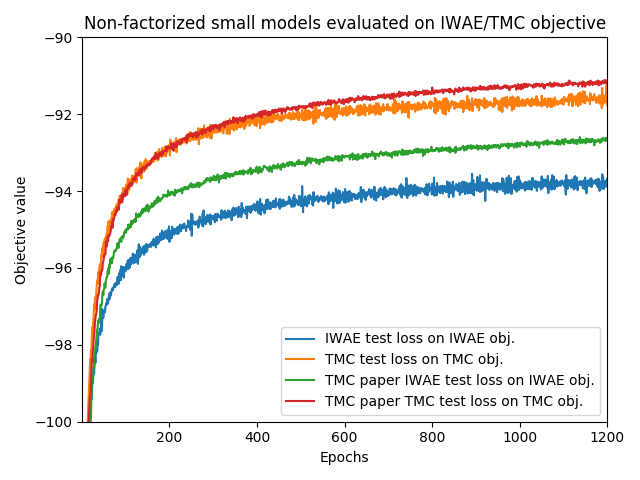
\includegraphics[height=5.5cm]{../openreview/Figures/nfs_iwae_tmc.png}
    \end{subfigure}%
    ~ 
    \begin{subfigure}[t]{0.5\textwidth}
        \centering
        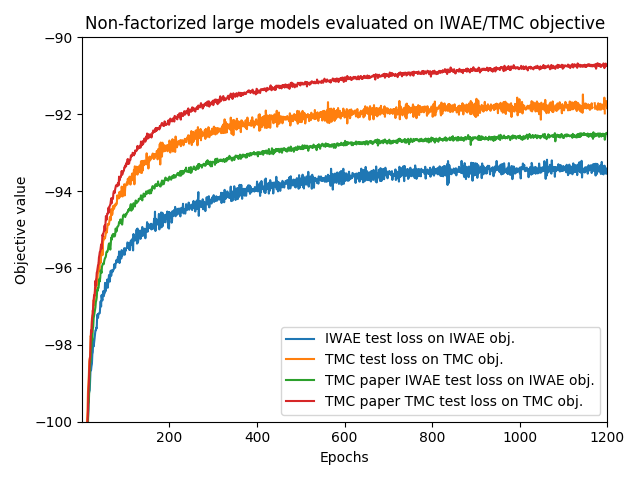
\includegraphics[height=5.5cm]{../openreview/Figures/nfl_iwae_tmc.png}
    \end{subfigure}
    \caption{Results of the non-factorized IWAE and TMC models, evaluated on their respective objective functions for both small and large models over 1200 epochs. Results corresponding to legends noted with ``TMC paper'' was given to us by the author. }
    \label{fig:iwae_tmc_small_large}
\end{figure*}

\begin{table}[ht!]
\centering
\begin{tabular}{|l|c|}
\hline
Model: & \multicolumn{1}{r|}{Mean objective value over last 50 epochs} \\ \hline
IWAE large & $-93.08\pm0.19$ \\ \hline
IWAE small & $-93.35\pm0.12$ \\ \hline
TMC large & $-91.94\pm0.12$ \\ \hline
TMC small & $-91.63\pm0.16$ \\ \hline
\end{tabular}
\caption{Reproduced results of the TMC and IWAE averaged over the last 50 epochs reported in negative log-likelihood (NLL). The values subsequent $\pm$ indicate standard deviation.}
\label{tab:50_ep_mean}
\end{table}

\begin{figure*}[th!]
    \centering
    \begin{subfigure}[t]{0.5\textwidth}
    \hspace*{-2cm}
        \centering
        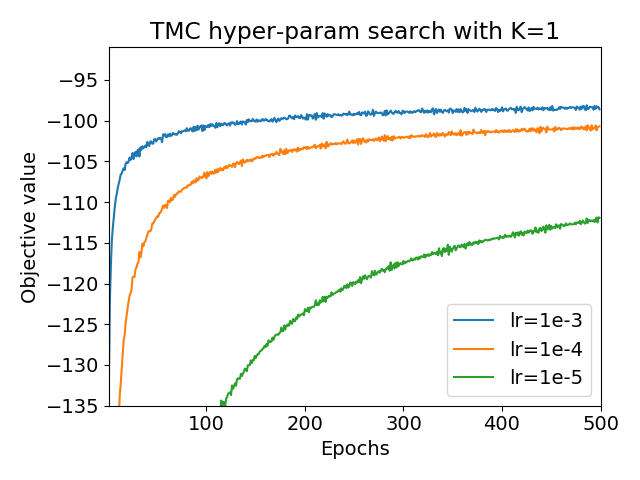
\includegraphics[height=5cm]{../openreview/Figures/hp_s_1.png}
    \end{subfigure}%
    ~ 
    \begin{subfigure}[t]{0.5\textwidth}
        \centering
        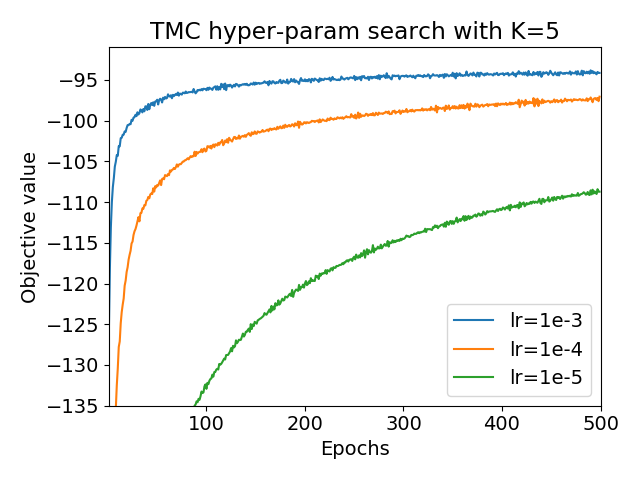
\includegraphics[height=5cm]{../openreview/Figures/hp_s_5.png}
    \end{subfigure}
        \begin{subfigure}[t]{0.5\textwidth}
    \hspace*{-2cm}
        \centering
        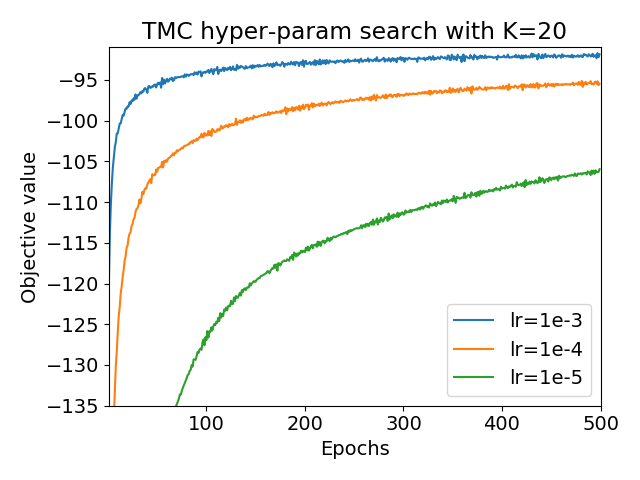
\includegraphics[height=5cm]{../openreview/Figures/hp_s_20.png}
    \end{subfigure}%
    ~ 
    \begin{subfigure}[t]{0.5\textwidth}
        \centering
        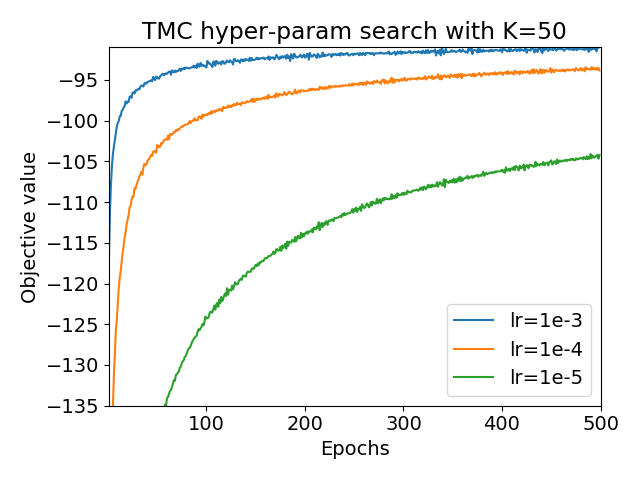
\includegraphics[height=5cm]{../openreview/Figures/hp_s_50.png}
    \end{subfigure}
    \caption{Results of the hyper-parameter search for the small TMC model, for different values of K and learning rates over 500 epochs.}
    \label{fig:hp_search}
\end{figure*}

The scores presented in Fig. \ref{fig:ablation_study} were obtained during our ablation study. We expected the two models to give similar results, as they, indeed, did. Averaged over an increasing number of runs, the results should become indistinguishable as TMC and IWAE are in essence the same algorithms when there is only one stochastic layer, i.e. no intermediate stochastic layers in contrast to the model shown in Fig. \ref{fig:tmc_layout}. This since the parameters of the prior distribution are fixed – the model assumes a standard normal distribution, therefor there is no new information when evaluating the latent variables under the same distribution parameters. To support this claim, we refer to Alg. \ref{algo:tmc}, specifically where we iterate through the distribution parameters. Mathematically, as is shown in \cite{tmc}, the number of evaluated importance samples grows exponentially with the layers, so if we reduce the number of layers to one, we effectively evaluate $K^1=K$ samples in the TMC, the same as for the IWAE. Regarding the worsening of the objective value after approximately 200 epochs, we are not sure how to explain this. Probably, it is due to the insufficiently small model (100 units per deterministic layer and one stochastic layer with four units). The purpose of our ablation study was simply to show that the TMC and IWAE are the same under the mentioned conditions, and so we do not dig deeper into this phenomena.

In Appendix \ref{sec:clusters}, we display the TMC's clustering abilities, compared to the IWAE, via a two-dimensional latent space. By observing Fig. \ref{fig:clusters}, it is clear that the TMC (right) yields less ambiguous clusters than those produced by the IWAE. Especially, note to which small degree digit nine's representation mixes with the others digit representations, as opposed to its cluster for the IWAE (left).

During our non-exhaustive hyper-parameter search, we evaluated the TMC model for $K\in\{1, 5, 20, 50\}$, and for each K we tested different learning rates $\text{lr}\in\{1e-5, 1e-4, 1e-3\}$. The results of this hyper-parameter search are presented in Fig. \ref{fig:hp_search}. Each of these different experiments was run over 500 epochs for the small TMC model, unsurprisingly $K=50$ with $\text{lr}=1e-3$ has the best performance over these 500 epochs. This as we are effectively looking at more samples for each batch. However, setting $K=50$ increases the running time significantly as the number of matrix calculations needed are more than doubled to that of $K=20$ and the performance is marginally better compared to that of setting $K=20$ and $\text{lr}=1e-3$. The parameter settings proposed in the TMC paper seems well suited for the previous experiments based on our hyper-parameter search. We also tested with $\text{lr}=1e-2$, and this produced NaN results for all different values of K we tested, this might be related to the inherent numerical instability of the TMC method, especially since we have not used weight normalization in our experiments. The deployment of weight normalization might very well alleviate this problem and a larger learning rate might be able to perform better than those we have examined. 


\begin{figure}[th!]
    \centering
    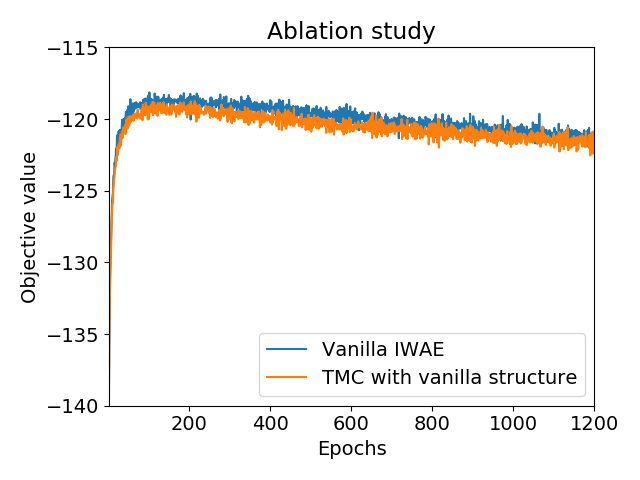
\includegraphics[width=0.5\textwidth, height=4.5cm]{../openreview/Figures/ablation_study_tmc.png}
    \caption{Results of the ablation study (more detailed description in text). The test was conducted with K=5, batch size=128 and a learning rate of 1e-3 over 500 epochs.}
    \label{fig:ablation_study}
\end{figure}
\section{Discussion and Conclusions}
Although our reproduced results and the TMC paper results differ,
the general observations of the authors remain valid. I.e., the TMC clearly outperforms the IWAE model on the given dataset. This is unsurprising as the TMC, for $K=20$ and five layers, considers a factor million more importance samples (\cite{tmc}). Despite this, we see that the author's claim concerning negligible time difference between the two models is also justifiable, according to our findings. We note in our work, that the intentions of \cite{tmc} were not to achieve state-of-the-art performances, but to compare the proposed the model to the baseline used in the TMC paper. Perhaps for this reason, the results are presented in a way such that they are impractical to study in detail. Although the author very skillfully and clearly describes the novelties in the TMC paper, understanding the model architecture was, for us, quite challenging. Furthermore, we argue that the specifics regarding the training and testing scheme could have been outlined in the TMC paper, at least for reproducibility.
We believe, the discrepancies in test results stems from two sources, us omitting the use of weight normalization, and the presented one-shot performances, i.e. non-averaged. 

To conclude, we have successfully reproduced the fundamental results of the NeurIPS 2019 paper "Tensor Monte Carlo: Particle Methods for the GPU Era", in order to support the author's claims. Additionally, we have complemented the original paper with an algorithmic description, a figure explaining the architecture and experiments displaying the TMC's reconstruction and clustering abilities. We applaud the author for an ingenious take to improve on the existing IWAE. We hope future work will be done on the tensor Monte-Carlo algorithm. 

\section{Acknowledgements}
We would like to thank Laurence Aitchison for supplying us with answers to our questions (patiently), and the original results so that we could integrate them here. 

% \bibliography{bibtex} 
% \bibliographystyle{ieeetr}